\chapter{Metodología y fase de análisis}\label{chap:3}

En este capítulo se describe, en primer lugar, la metodología de desarrollo utilizada y, posteriormente, se detalla el análisis previo al diseño, que comprende el escenario de uso, los requisitos que debe satisfacer el protocolo y la viabilidad técnica, económica y legal del trabajo.

Dado que este proyecto consiste en el diseño de un protocolo de comunicaciones, cuyo comportamiento depende de un canal de radio compartido y con pérdidas, no se ha seguido un modelo de desarrollo en cascada, en el que el diseño se cierra por completo antes de implementar y la validación se deja para el final. En un protocolo, buena parte de los problemas (colisiones, temporizadores mal dimensionados o interacciones inesperadas entre tramas) solo se manifiestan cuando el código se ejecuta, por lo que cualquier hallazgo durante la validación obliga a revisar el diseño.

Por este motivo, se ha seleccionado un modelo de desarrollo iterativo e incremental. No se ha aplicado de manera formal ninguna metodología ágil concreta, como podría ser Scrum, aunque sí se han adoptado sus principios básicos: incrementos pequeños y funcionales, y verificación continua.

\section{Metodología de desarrollo}\label{sec:metodologia}

El modelo iterativo e incremental divide el desarrollo en ciclos cortos, cada uno de los cuales añade una funcionalidad concreta sobre una versión del sistema que ya funciona. En este trabajo, cada iteración se compone de cuatro actividades: análisis, diseño, implementación y verificación. En el análisis se identifican la funcionalidad que se va a incorporar y los requisitos a los que responde. En el diseño se definen los elementos que forman parte del protocolo: formato de paquete, mecanismos de sincronización, políticas de reintentos, etc. En la implementación se codifica el incremento en la librería. Por último, en la verificación se comprueba el incremento y se revisa que no haya alterado el comportamiento de lo ya construido.

\section{Análisis del sistema en el que se basa el protocolo}\label{sec:escenario}

Como se ha comentado, el objetivo de este trabajo es desarrollar un protocolo de comunicación de área local sobre la capa física de LoRa para una aplicación concreta.

El sistema a desarrollar es una aplicación de registro de clases y monitoreo de aulas. Con esta herramienta, se pretende proporcionar a los profesores un sistema que permita registrar sus clases empleando una tarjeta NFC de forma más sencilla. Actualmente, se emplea un portal web al que los docentes deben acceder mediante certificado digital para registrar las clases. Por otro lado, se pretende recoger información sobre las aulas, como la humedad, la temperatura, la luminosidad y detección de presencia. Con esto se proporciona a los conserjes una herramienta que les permita monitorear las aulas de un vistazo con la capacidad de gestionar remotamente el sistema de climatización y las persianas. 

El escenario de referencia es un edificio, concretamente el aulario del centro universitario, con una veintena de aulas repartidas en dos plantas. Las distancias entre cualquier aula y un punto central del edificio son de decenas de metros, con muros intermedios. Los dispositivos están alimentados desde la red eléctrica, por lo que el consumo no es, en principio, una restricción relevante.

En este escenario intervienen los siguientes elementos:

\begin{itemize}
\item \textbf{Nodo de aula}: Dispositivo instalado en cada aula, con lector NFC, sensores ambientales y relés.
\item \textbf{Gateway}: Dispositivo único del sistema que gestiona la red de nodos, con conexión hacia el servidor y capacidad de alojar en local el propio servidor y la base de datos.
\item \textbf{Servidor web}: Aloja la lógica de la aplicación y la base de datos, y queda fuera de la red de radio.
\item \textbf{Usuarios}: Habrá tres tipos de usuarios del sistema: profesores, conserjes y administradores.
\end{itemize}

El escenario genera tres clases de tráfico con exigencias muy distintas, que son las que determinan el diseño del acceso al medio. En la Tabla~\ref{tab:trafico} se muestran dichas clases.

\begin{table}[htbp]
\centering
\caption{Clases de tráfico del escenario de uso.}\label{tab:trafico}
\renewcommand{\arraystretch}{1.3}
\begin{tabularx}{\textwidth}{p{2.4cm} p{2.4cm} p{2.4cm} X}
\toprule
\textbf{Tráfico} & \textbf{Sentido} & \textbf{Patrón} & \textbf{Exigencia} \\
\midrule
Evento (fichaje) & Nodo $\rightarrow$ gateway, con respuesta & Esporádico e imprevisible & Respuesta al usuario del orden de un segundo. No puede perderse, falsificarse ni duplicarse. \\
\midrule
Telemetría (sensores, estado) & Nodo $\rightarrow$ gateway & Periódico & Tolera retardos de decenas de segundos y la pérdida ocasional de una muestra. \\
\midrule
Órdenes (relés, reinicio) & Gateway $\rightarrow$ nodo & Esporádico & Efecto en pocos segundos. Debe confirmarse. \\
\bottomrule
\end{tabularx}
\end{table}

Como se observa en la Tabla~\ref{tab:trafico}, el tráfico periódico es predecible y admite planificación, mientras que el evento es urgente pero infrecuente y la orden exige que el nodo sea alcanzable en cualquier momento. Por tanto, ningún esquema de acceso único sirve adecuadamente a las tres clases.

\subsection{Requisitos del sistema}

Los requisitos funcionales del sistema se agrupan en cinco bloques.

El primero es el fichaje. El profesor ficha acercando su tarjeta NFC al nodo del aula \textbf{(SIS-1)}. El servidor valida el fichaje comprobando que la tarjeta esté registrada, que el nodo tenga un aula asignada, que haya una clase en curso y que esa clase sea de ese profesor \textbf{(SIS-2)}. El nodo recibe el resultado, que puede ser OK, sin clase, denegado, desconocido o reintentar \textbf{(SIS-3)}, y el sistema garantiza que ningún fichaje se pierda ni se registre dos veces \textbf{(SIS-4)}.

El segundo bloque es la monitorización del aula. El nodo mide temperatura, humedad, presión, luz y presencia, y envía los datos periódicamente \textbf{(SIS-5)}. El conserje y el administrador pueden ver el estado de cada aula y si su nodo está en línea \textbf{(SIS-6)}.

El tercero es el control remoto. El conserje y el administrador pueden encender y apagar la calefacción y la iluminación de un aula \textbf{(SIS-7)}. Además, el administrador puede reiniciar los nodos y asignarles un aula \textbf{(SIS-8)}.

El cuarto es la gestión de datos y usuarios. El administrador gestiona usuarios, aulas, clases y asistencias \textbf{(SIS-9)}, y el profesor consulta su historial de asistencias \textbf{(SIS-10)}. Los usuarios inician sesión con correo y contraseña, y cada rol accede a su propio panel \textbf{(SIS-11)}.

Por último, el sistema obtiene el horario de clases de la base de datos y, si no está disponible allí, lo solicita al servicio de reservas de la universidad \textbf{(SIS-12)}.

\section{Especificación de requisitos del protocolo LoRaLAN}\label{sec:requisitos}

Tras la recogida de requisitos del sistema de registro de clases y monitoreo de aulas, se procede a la elaboración de la especificación de requisitos del protocolo a desarrollar. 

\subsection{Requisitos funcionales}

\begin{longtable}{@{}l p{0.26\textwidth} p{0.52\textwidth}@{}}
\caption{Requisitos funcionales del protocolo LoRaLAN.}\label{tab:pro}\\
\toprule
\textbf{ID} & \textbf{Requisito} & \textbf{Descripción} \\
\midrule
\endfirsthead
\toprule
\textbf{ID} & \textbf{Requisito} & \textbf{Descripción} \\
\midrule
\endhead
\bottomrule
\endfoot
PRO-1 & Comunicación entre nodos y gateway & El protocolo debe permitir la comunicación entre un gateway y múltiples nodos pertenecientes a una misma red. \\
\midrule
PRO-2 & Transmisión de telemetría & El protocolo debe permitir que los nodos transmitan datos de telemetría al gateway de forma periódica y que el gateway detecte los nodos inactivos. \\
\midrule
PRO-3 & Comunicación de eventos asíncronos & El protocolo debe permitir que los nodos comuniquen eventos al gateway sin depender exclusivamente de la comunicación periódica, comprobando previamente que el canal esté libre, y que reciban en la confirmación un código de estado de la aplicación. \\
\midrule
PRO-4 & Comunicación descendente & El protocolo debe permitir que el gateway envíe órdenes y mensajes dirigidos a nodos concretos, de modo que una orden se ejecute como mucho una vez. \\
\midrule
PRO-5 & Confirmación de entrega & El protocolo debe confirmar la recepción de los mensajes que lo requieran, de modo que la confirmación garantice la entrega. Ante la falta de confirmación, debe retransmitir un número acotado de veces, informar a la aplicación si no logra la entrega y permitir que un evento se entregue por la vía del sondeo. \\
\midrule
PRO-6 & Gestión de la incorporación y salida de nodos & El protocolo debe permitir la incorporación autenticada de nodos a la red y su posterior salida de forma controlada. \\
\midrule
PRO-7 & Sincronización temporal & El protocolo debe permitir distribuir referencias temporales desde el gateway a los nodos. \\
\midrule
PRO-8 & Seguridad de las comunicaciones & El protocolo debe proporcionar mecanismos que garanticen la confidencialidad, autenticidad e integridad de los mensajes, además de protección frente a repetición. \\
\midrule
PRO-9 & Recuperación ante la pérdida del gateway & Un nodo asociado debe detectar la ausencia prolongada de tráfico dirigido a él y volver a asociarse sin reiniciarse. El plazo de detección debe ser configurable y superior al tiempo entre dos turnos de sondeo del nodo. \\
\end{longtable}

\subsection{Requisitos no funcionales}
\begin{table}[htbp]
    \centering
    \caption{Requisitos no funcionales del protocolo.}
    \label{tab:requisitos-no-funcionales}
    \renewcommand{\arraystretch}{1.3}
    \begin{tabularx}{\textwidth}{l l X}
        \toprule
        \textbf{ID} & \textbf{Requisito} & \textbf{Descripción} \\
        \midrule
        RNF-1 & Eficiencia & El protocolo debe minimizar la latencia de las comunicaciones y el tiempo de ocupación del canal radio. \\\midrule
        RNF-2 & Cumplimiento normativo & El funcionamiento debe respetar las restricciones de uso radioeléctrico aplicables a la sub-banda seleccionada~\cite{etsien3002202,ercrec7003}. \\ \midrule
        RNF-3 & Recursos y capacidad & La implementación debe funcionar sobre hardware de bajo coste, utilizar memoria estática y admitir al menos 32 nodos mediante estructuras de tamaño fijo. La carga útil de las tramas no debe superar los 64~bytes. \\ \midrule
        RNF-4 & Portabilidad e integración & El protocolo debe implementarse como una librería independiente de la aplicación y adaptable a distintos transceptores compatibles, con una interfaz sencilla de utilizar. \\ \midrule
        RNF-5 & Verificabilidad & La lógica del protocolo debe poder probarse de forma determinista y repetible sin necesidad de hardware físico. \\ 
        \bottomrule
    \end{tabularx}
\end{table}

\section{Caracterización del espectro con radio definida por software}\label{sec:sdr}

Antes de diseñar y desarrollar el protocolo se debe confirmar que el canal de radio en la localización donde se desplegaría no está excesivamente ocupado, ya que un canal con mucho tráfico degradaría la calidad de la conexión provocando colisiones. 


Por tanto, se midió la ocupación real de la banda en la que puede operar LoRa en el aulario, empleando para ello una radio definida por software HackRF One~\cite{hackrfone}. El objetivo es, por un lado, determinar la actividad existente, ya que en el centro opera un gateway LoRaWAN, y, por otro lado, localizar la sub-banda disponible que más conviene para este sistema. A continuación, se introduce la banda en la que opera LoRa en Europa.

\subsection{Bandas ISM y de dispositivos de corto alcance}
\label{subsec:banda-ism}

Las bandas ISM son fragmentos del espectro radioeléctrico que la Unión Internacional de Telecomunicaciones (UIT) reservó para aplicaciones industriales, científicas y médicas. Se han consolidado como el espacio habitual para comunicaciones de uso libre porque no requieren licencia. Para operar en ellas, los equipos deben cumplir unas condiciones técnicas comunes y aceptar las interferencias sin derecho a protección~\cite{uitrr}.

En Europa, LoRa opera en la banda de 863--870~MHz (EU868). Aunque suele llamarse ISM, en sentido estricto es una banda para dispositivos de corto alcance (SRD, \textit{Short Range Devices}). Su uso está definido en la Unión Europea por la Decisión 2006/771/CE y sus modificaciones~\cite{decision2006771,decision20191345}, de obligado cumplimiento para los Estados miembros, que en España se aplica a través del Cuadro Nacional de Atribución de Frecuencias (CNAF)~\cite{cnaf2026}. Los equipos deben cumplir además la norma técnica ETSI EN~300~220~\cite{etsien3002202}. La banda se divide en sub-bandas con límites de potencia radiada aparente (PRA)\footnote{Potencia que un transmisor entrega a la antena multiplicada por la ganancia de dicha antena, en una dirección determinada, tomando como referencia un dipolo de media onda~\cite{raing_pra}.} y de ciclo de trabajo (\textit{duty cycle}), es decir, la fracción máxima de tiempo por hora que un dispositivo puede transmitir. Como alternativa al ciclo de trabajo, se pueden usar mecanismos de escucha previa y agilidad de frecuencia (LBT+AFA, \textit{Listen Before Talk} y \textit{Adaptive Frequency Agility}) como requisitos para operar en estas bandas. La Tabla~\ref{tab:subbandas-868} resume las principales sub-bandas~\cite{ercrec7003}.
\begin{table}[htbp]
    \centering
    \caption{Principales sub-bandas de la banda de 868~MHz para dispositivos de corto alcance de uso genérico~\cite{ercrec7003}.}
    \label{tab:subbandas-868}
    \renewcommand{\arraystretch}{1.3}
    \begin{tabular}{l c c}
        \toprule
        \textbf{Rango de frecuencias} & \textbf{PRA máxima} & \textbf{Ciclo de trabajo} \\
        \midrule
        863,0--865,0~MHz & 25~mW & 0,1\,\% \\
        865,0--868,0~MHz & 25~mW & 1\,\% \\
        868,0--868,6~MHz & 25~mW & 1\,\% \\
        868,7--869,2~MHz & 25~mW & 0,1\,\% \\
        869,4--869,65~MHz & 500~mW & 10\,\% \\
        869,7--870,0~MHz & 5~mW / 25~mW & Sin límite / 1\,\% \\
        \bottomrule
    \end{tabular}
\end{table}

Inicialmente, lo ideal sería desplegar el sistema sobre la sub-banda de 869,4--869,65~MHz, ya que es la menos restrictiva, aunque no puede afirmarse que sea la mejor opción sin medir el uso del canal.

\subsection{El procedimiento empleado para la medición}

Se definió un único punto de medida, situado en el aulario, que es el escenario objetivo. Se realizó una captura larga, de una hora ininterrumpida, puesto que esta duración es necesaria para estimar la ocupación de transmisores esporádicos.

Para la medición se empleó la herramienta \texttt{hackrf\_sweep}, que barre repetidamente el rango indicado y vuelca a un fichero de texto la potencia medida en cada intervalo de frecuencia. La resolución fue de 98~kHz por intervalo, del orden del ancho de un canal LoRa de 125~kHz. La captura larga del aulario se realizó el 5 de febrero de 2026, entre las 11:41 y las 12:41, y contiene un total de 1\,464\,485 barridos de la banda.

\begin{figure}[htbp]
    \centering
    \begin{subfigure}[b]{0.48\textwidth}
        \centering
        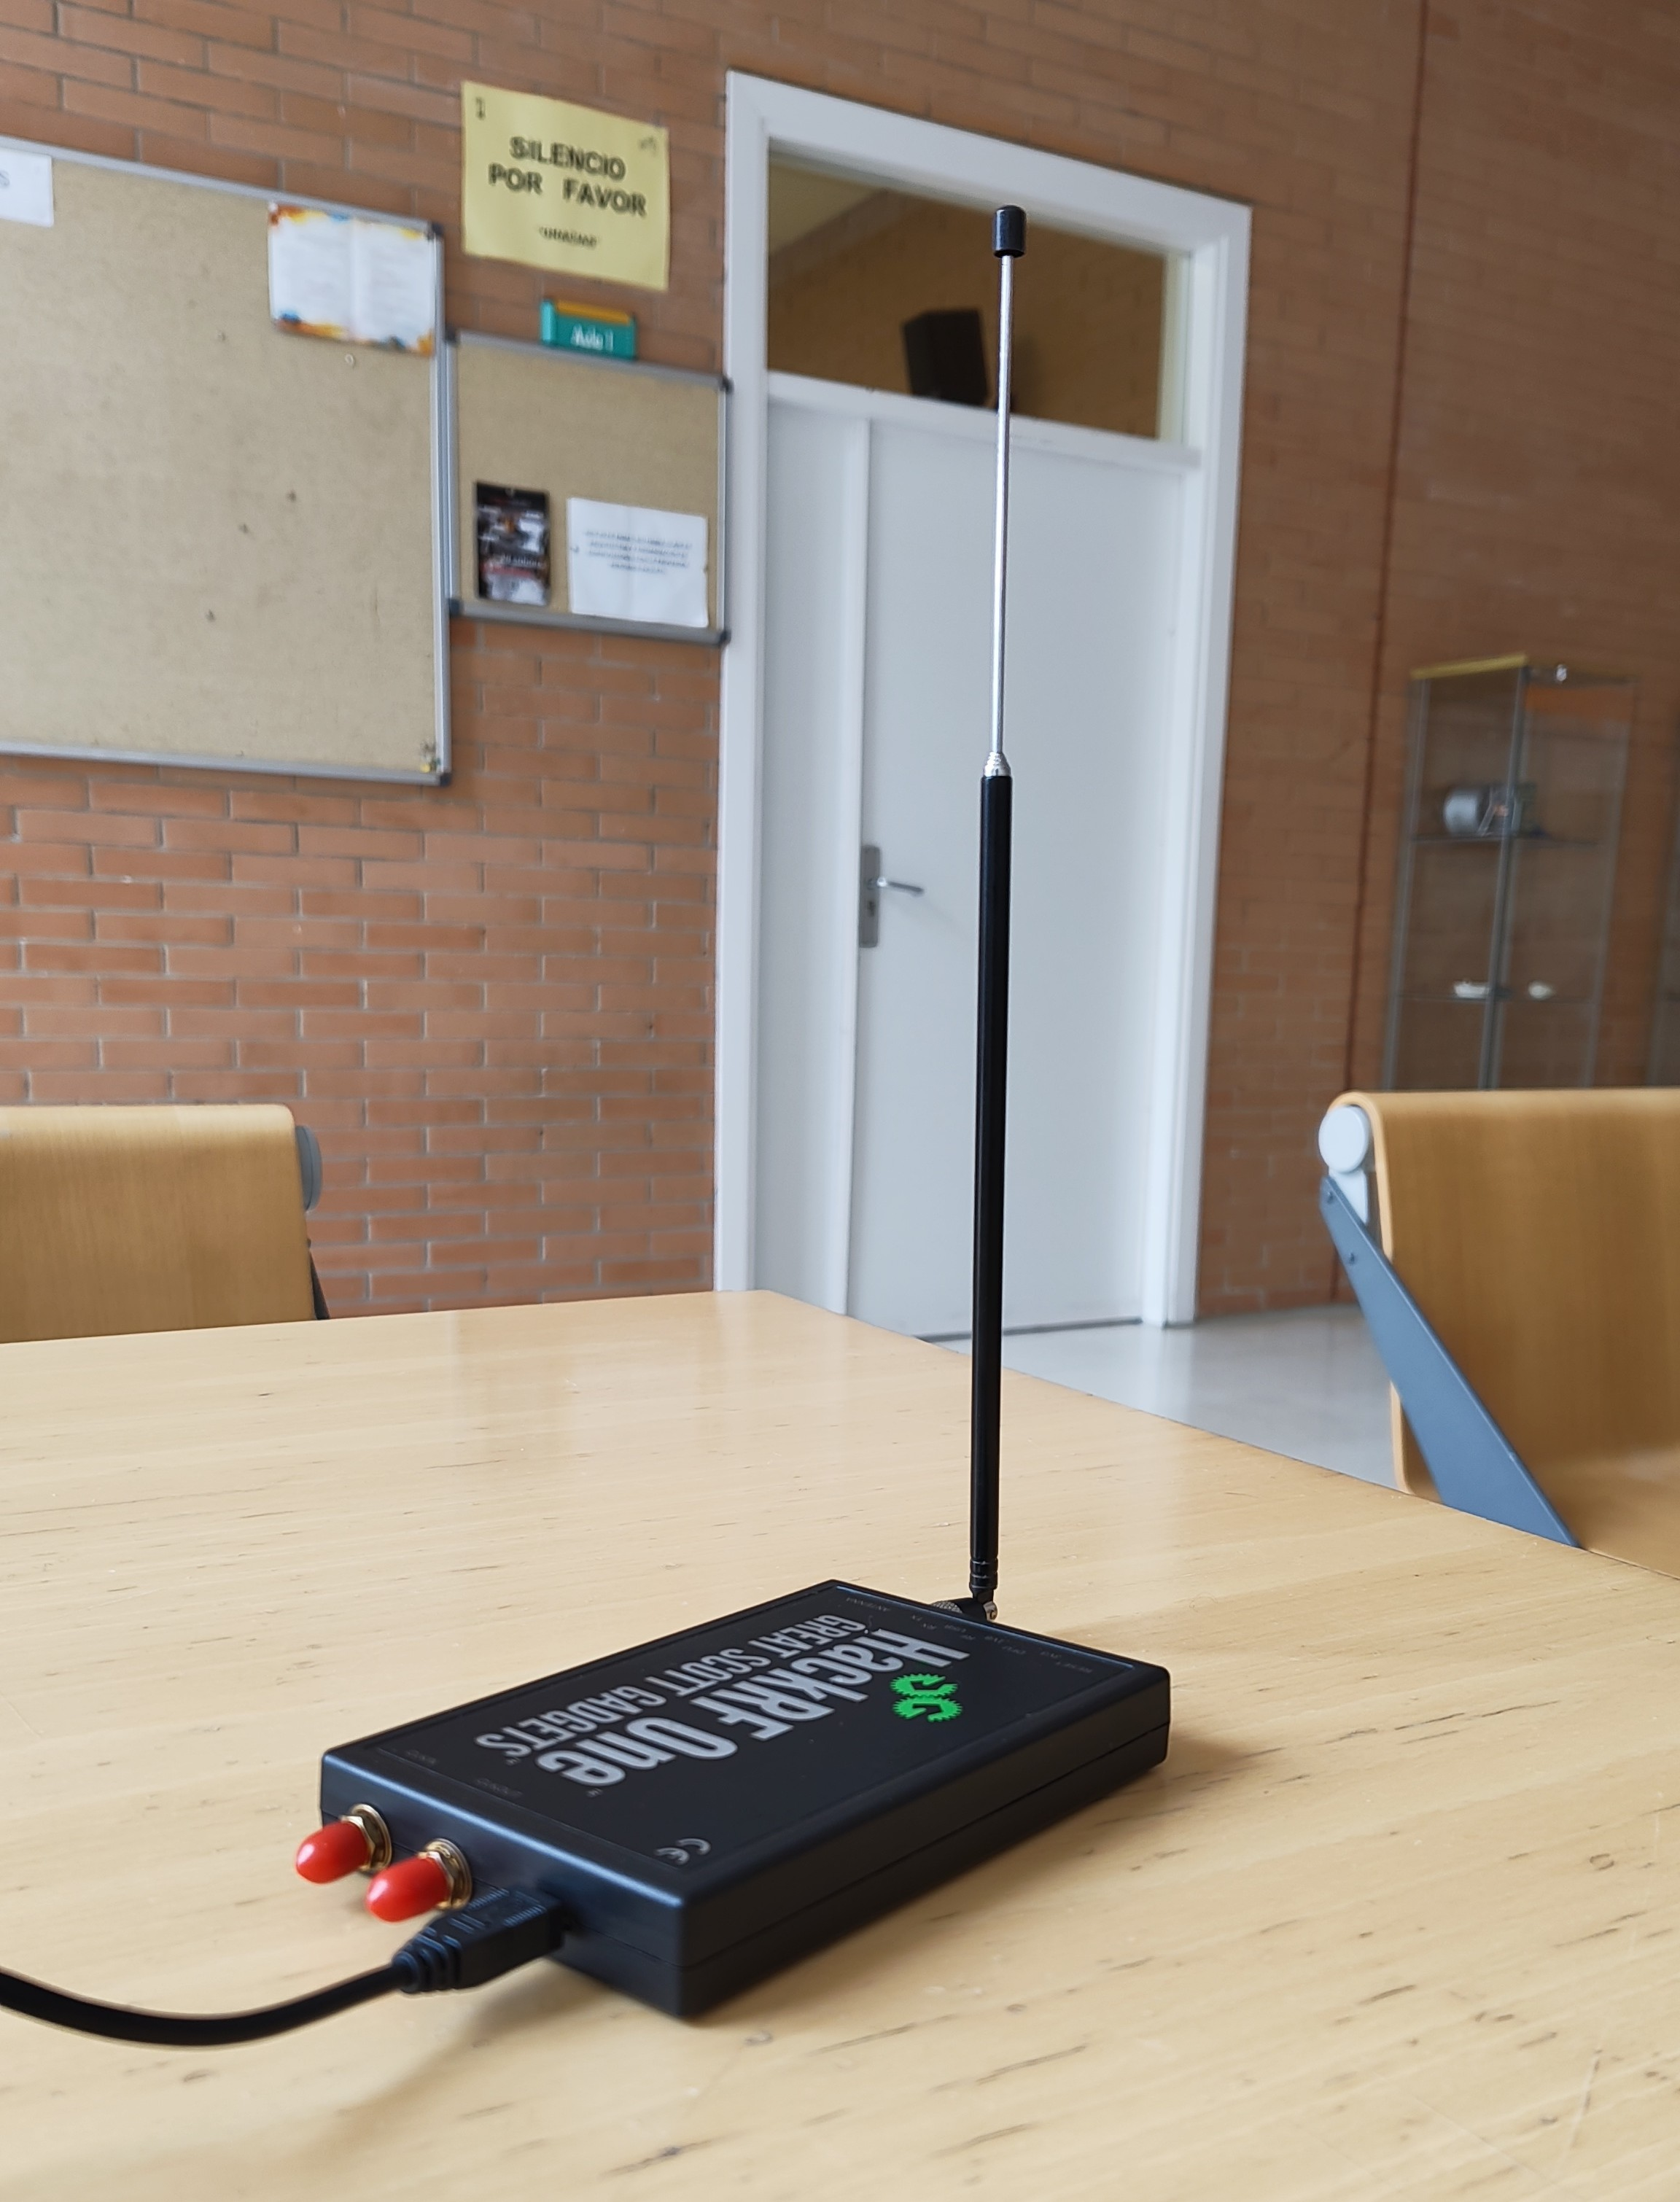
\includegraphics[width=\textwidth]{imagenes/sdr.jpg}
        \caption{Montaje empleado para la medición}
        \label{fig:sdr}
    \end{subfigure}
    \hfill
    \begin{subfigure}[b]{0.48\textwidth}
        \centering
        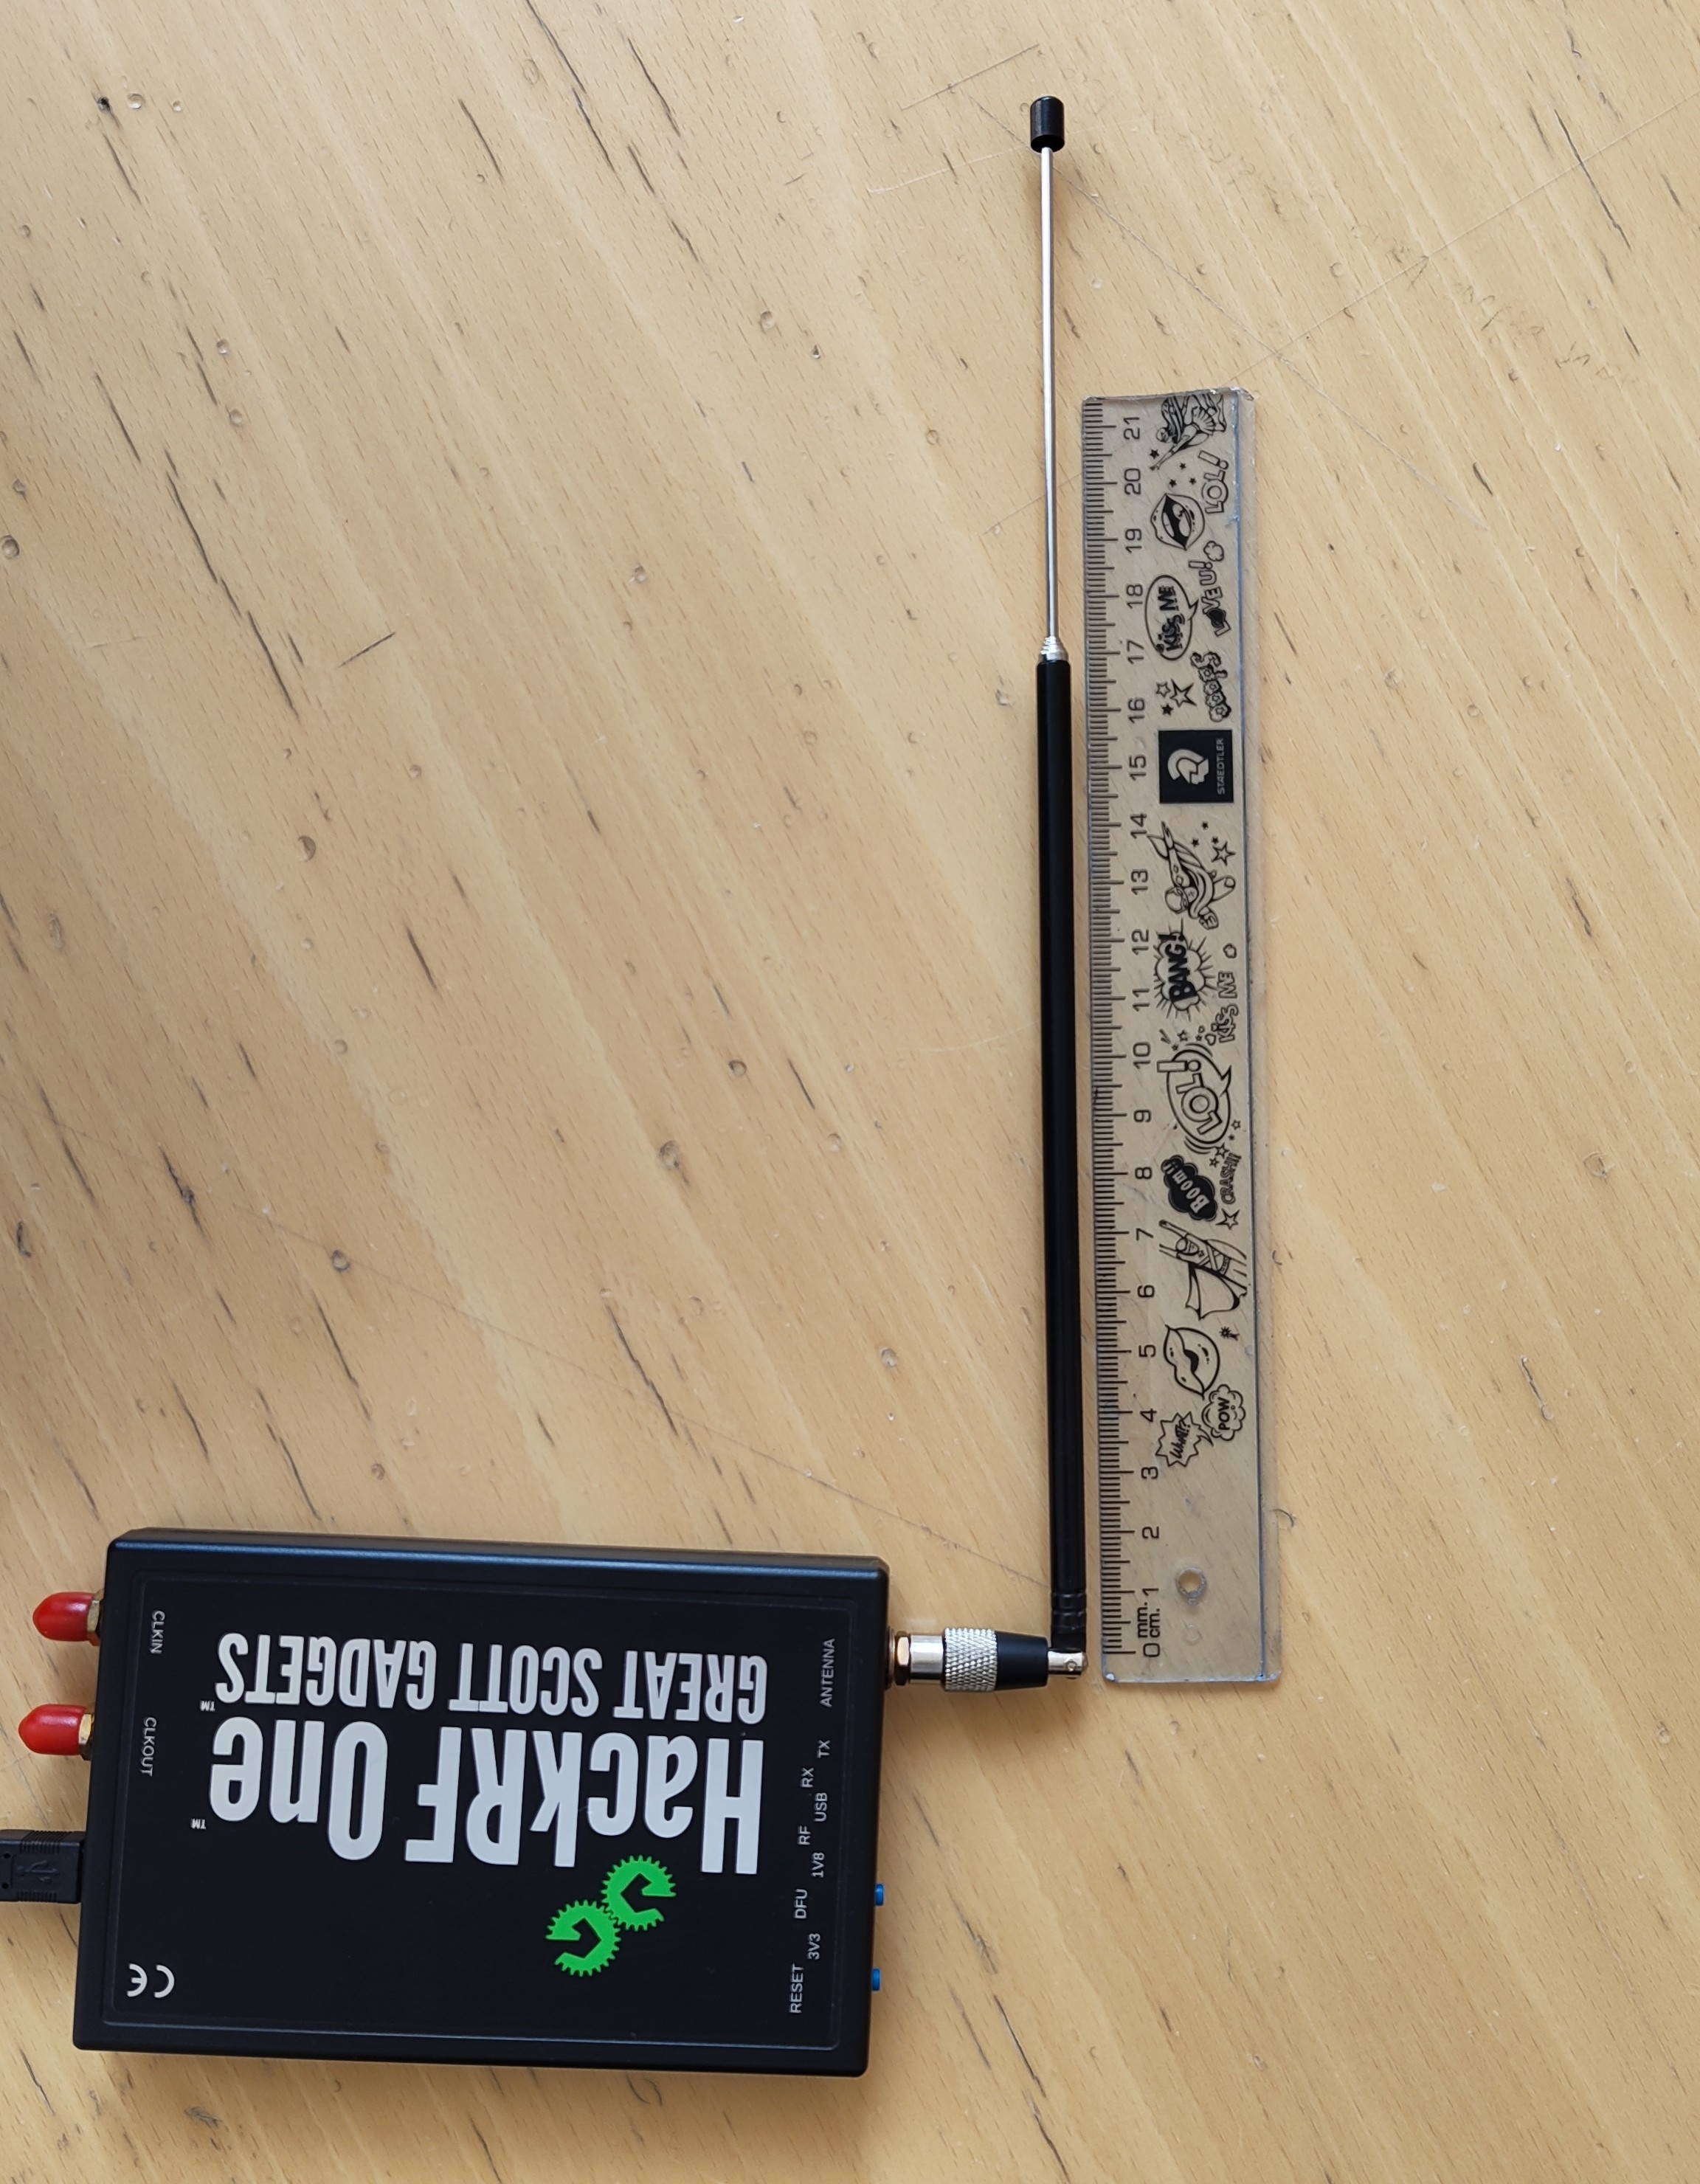
\includegraphics[width=\textwidth]{imagenes/sdr2.jpg}
        \caption{Medición de la antena telescópica}
        \label{fig:sdr2}
    \end{subfigure}
    \caption{Medición del espectro con HackRF One en el aulario.}
    \label{fig:conjunto}
\end{figure}

En la Figura~\ref{fig:sdr} se muestra el montaje realizado. Aunque no se puede apreciar en la imagen, la antena telescópica mide 26~cm. Esta antena funciona como un monopolo, que resuena cuando su longitud es un múltiplo impar de un cuarto de la longitud de onda ($\lambda/4$). A la frecuencia de trabajo, de aproximadamente 868~MHz, la longitud de onda es:

\begin{equation}
    \lambda = \frac{c}{f} = \frac{3 \cdot 10^{8}~\text{m/s}}{868 \cdot 10^{6}~\text{Hz}} \approx 34{,}6~\text{cm}
\end{equation}

Por ello, la antena se ajustó a una longitud de $3\lambda/4 \approx 26$~cm. Con esta longitud se mejora la adaptación de impedancias con el receptor y se reducen las pérdidas por reflexión.


El procesado se realizó mediante un \textit{script} en Python (Pandas, NumPy y Matplotlib), calculando sobre los datos obtenidos las tres métricas siguientes:

\begin{itemize}
\item \textbf{Potencia de ruido}: Potencia media de cada intervalo en ausencia de transmisiones.

\item \textbf{Valor máximo (\textit{max hold})}: Mayor potencia registrada en cada intervalo durante toda la captura. Revela transmisores potentes o cercanos, aunque emitan durante poco tiempo.

\item \textbf{Ocupación}: Porcentaje de barridos en los que la potencia de un intervalo supera un umbral situado por encima del ruido, fijado en $-55$~dBFS (unos 12~dB sobre el piso).
\end{itemize}

Las potencias se expresan en dBFS, es decir, son relativas al fondo de escala del conversor de la radio. Como el HackRF no está calibrado en potencia absoluta, las cifras son válidas para comparar frecuencias entre sí, pero no como medidas en dBm.

\subsection{Resultados y conclusiones de las mediciones}

En la Figura~\ref{fig:espectro} se resume la captura de una hora realizada en el aulario.
\begin{figure}[htbp]
\centering
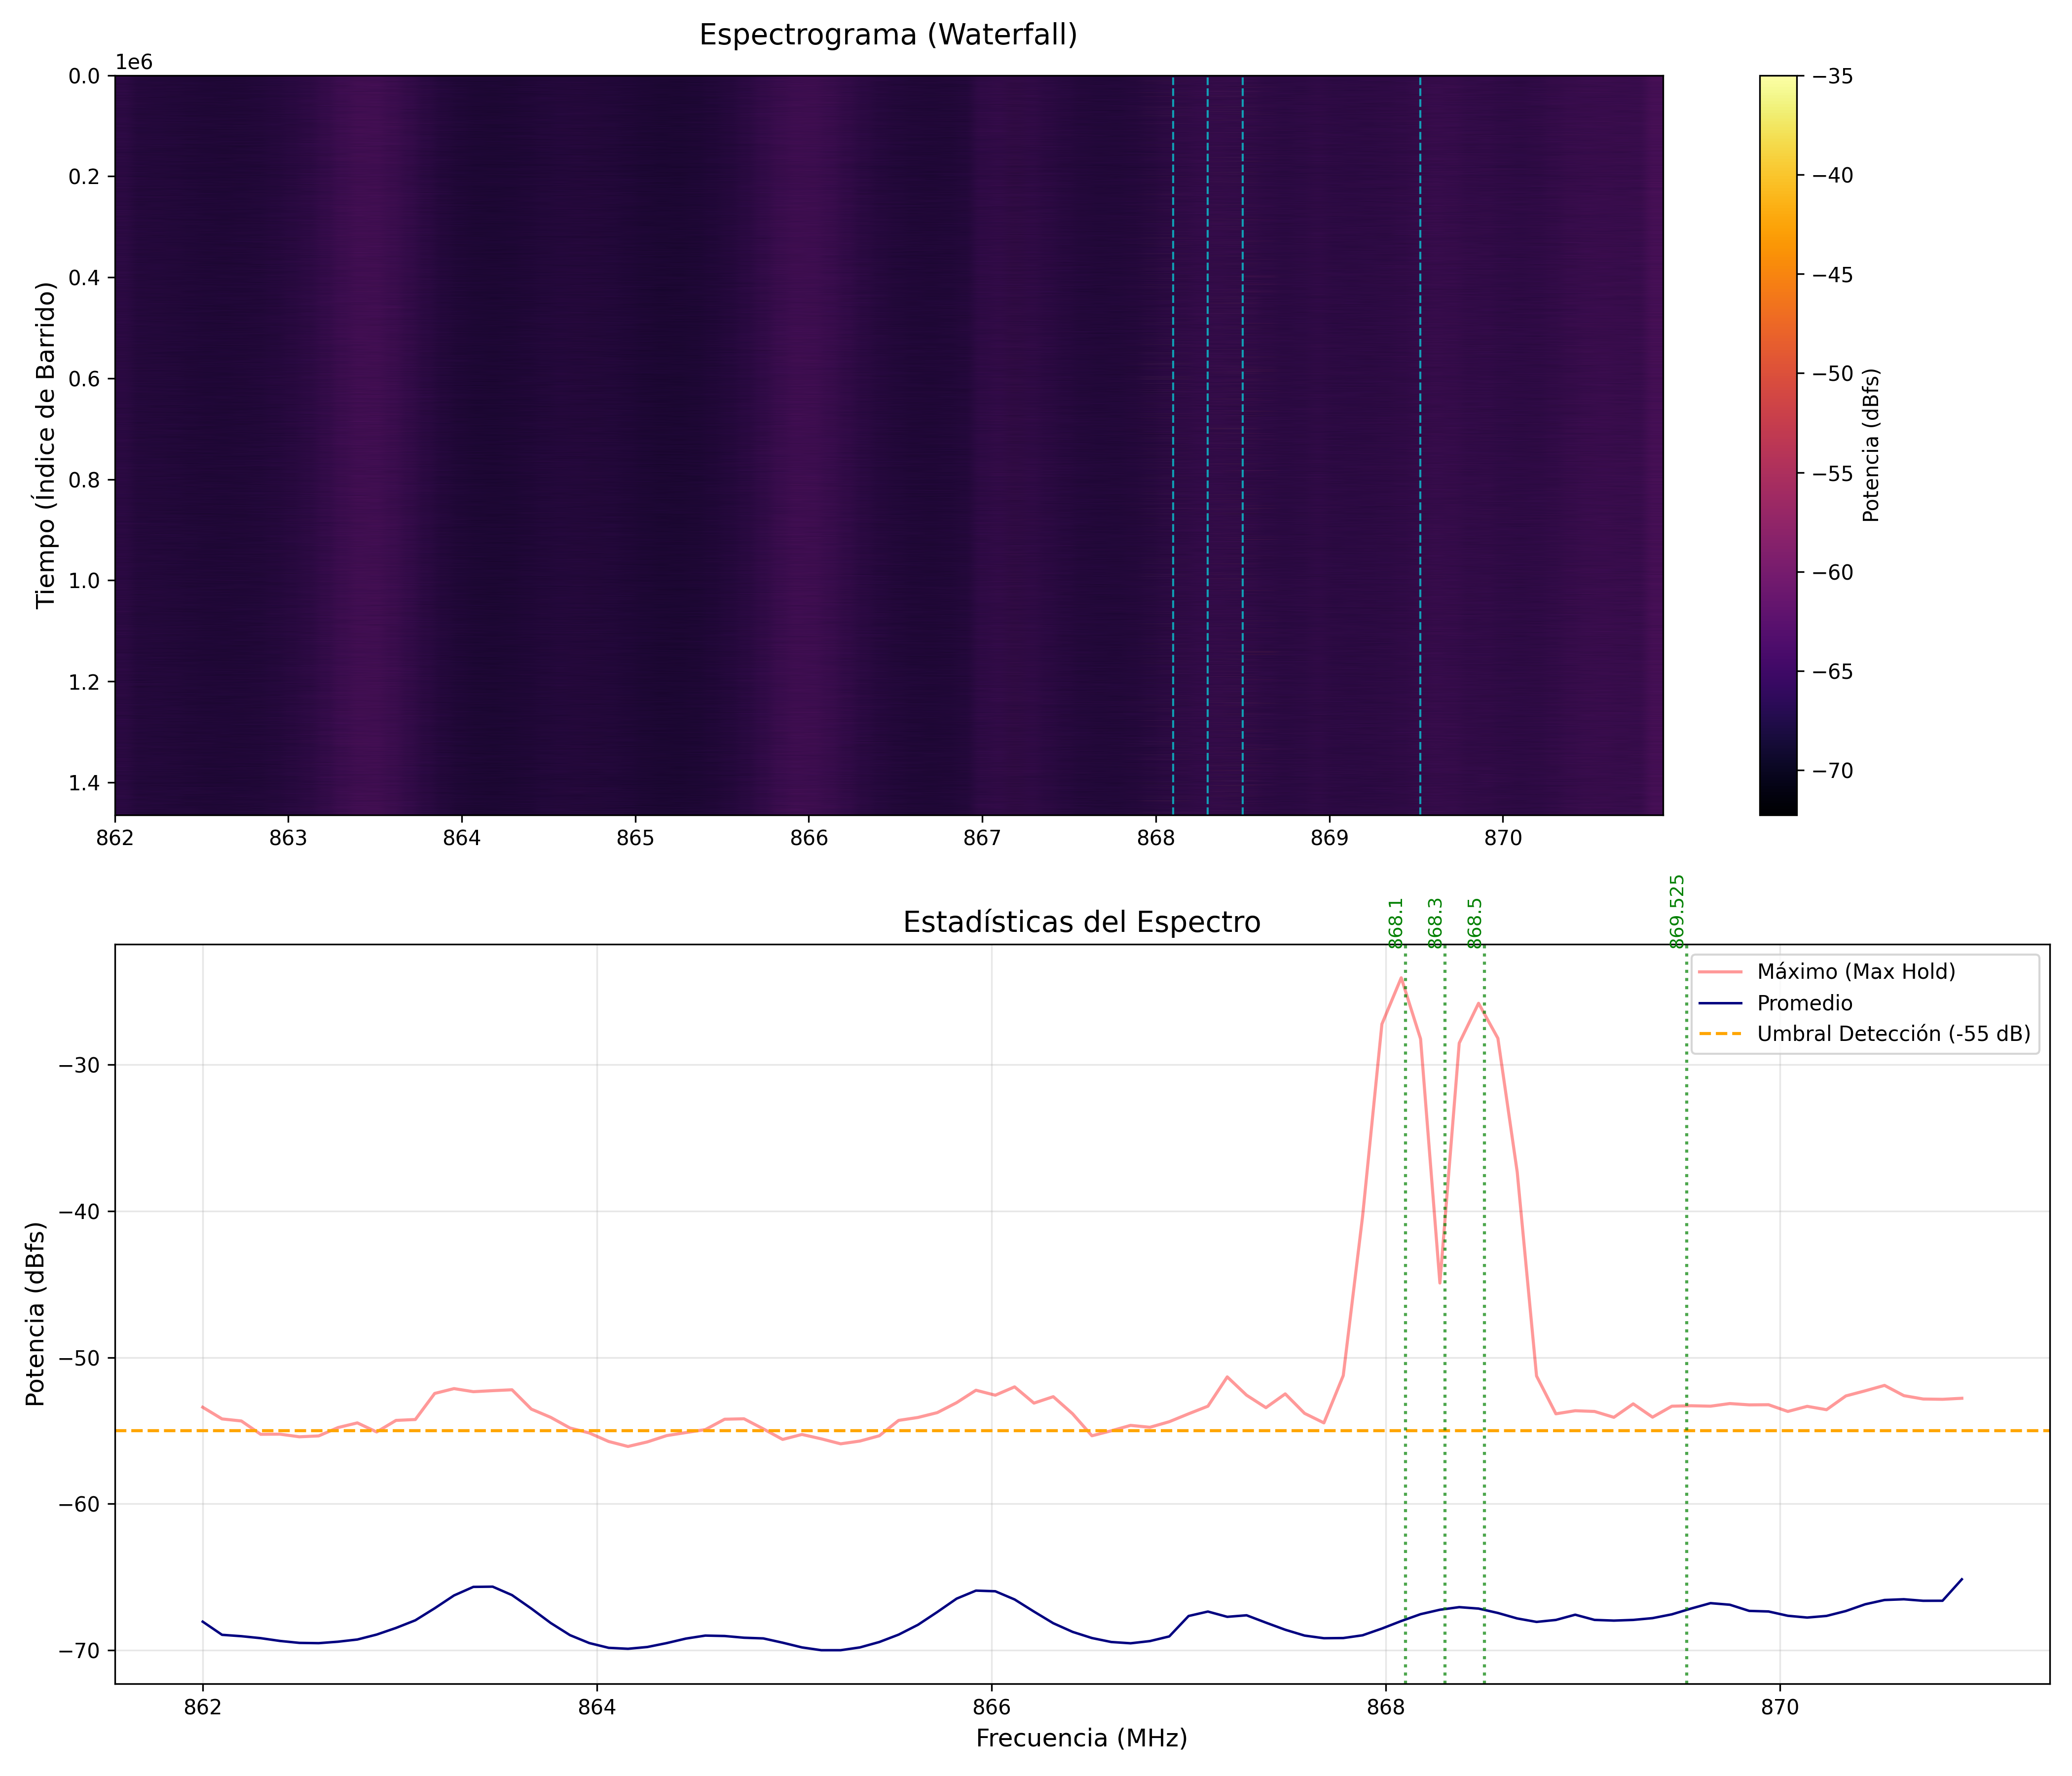
\includegraphics[width=\textwidth]{imagenes/analisis_lora_vertical_prueba.png}
\caption{\label{fig:espectro} Captura de una hora en el aulario (863--870~MHz). Arriba: espectrograma. Abajo: valor máximo y valor medio por frecuencia.}
\end{figure}

\begin{figure}[htbp]
\centering
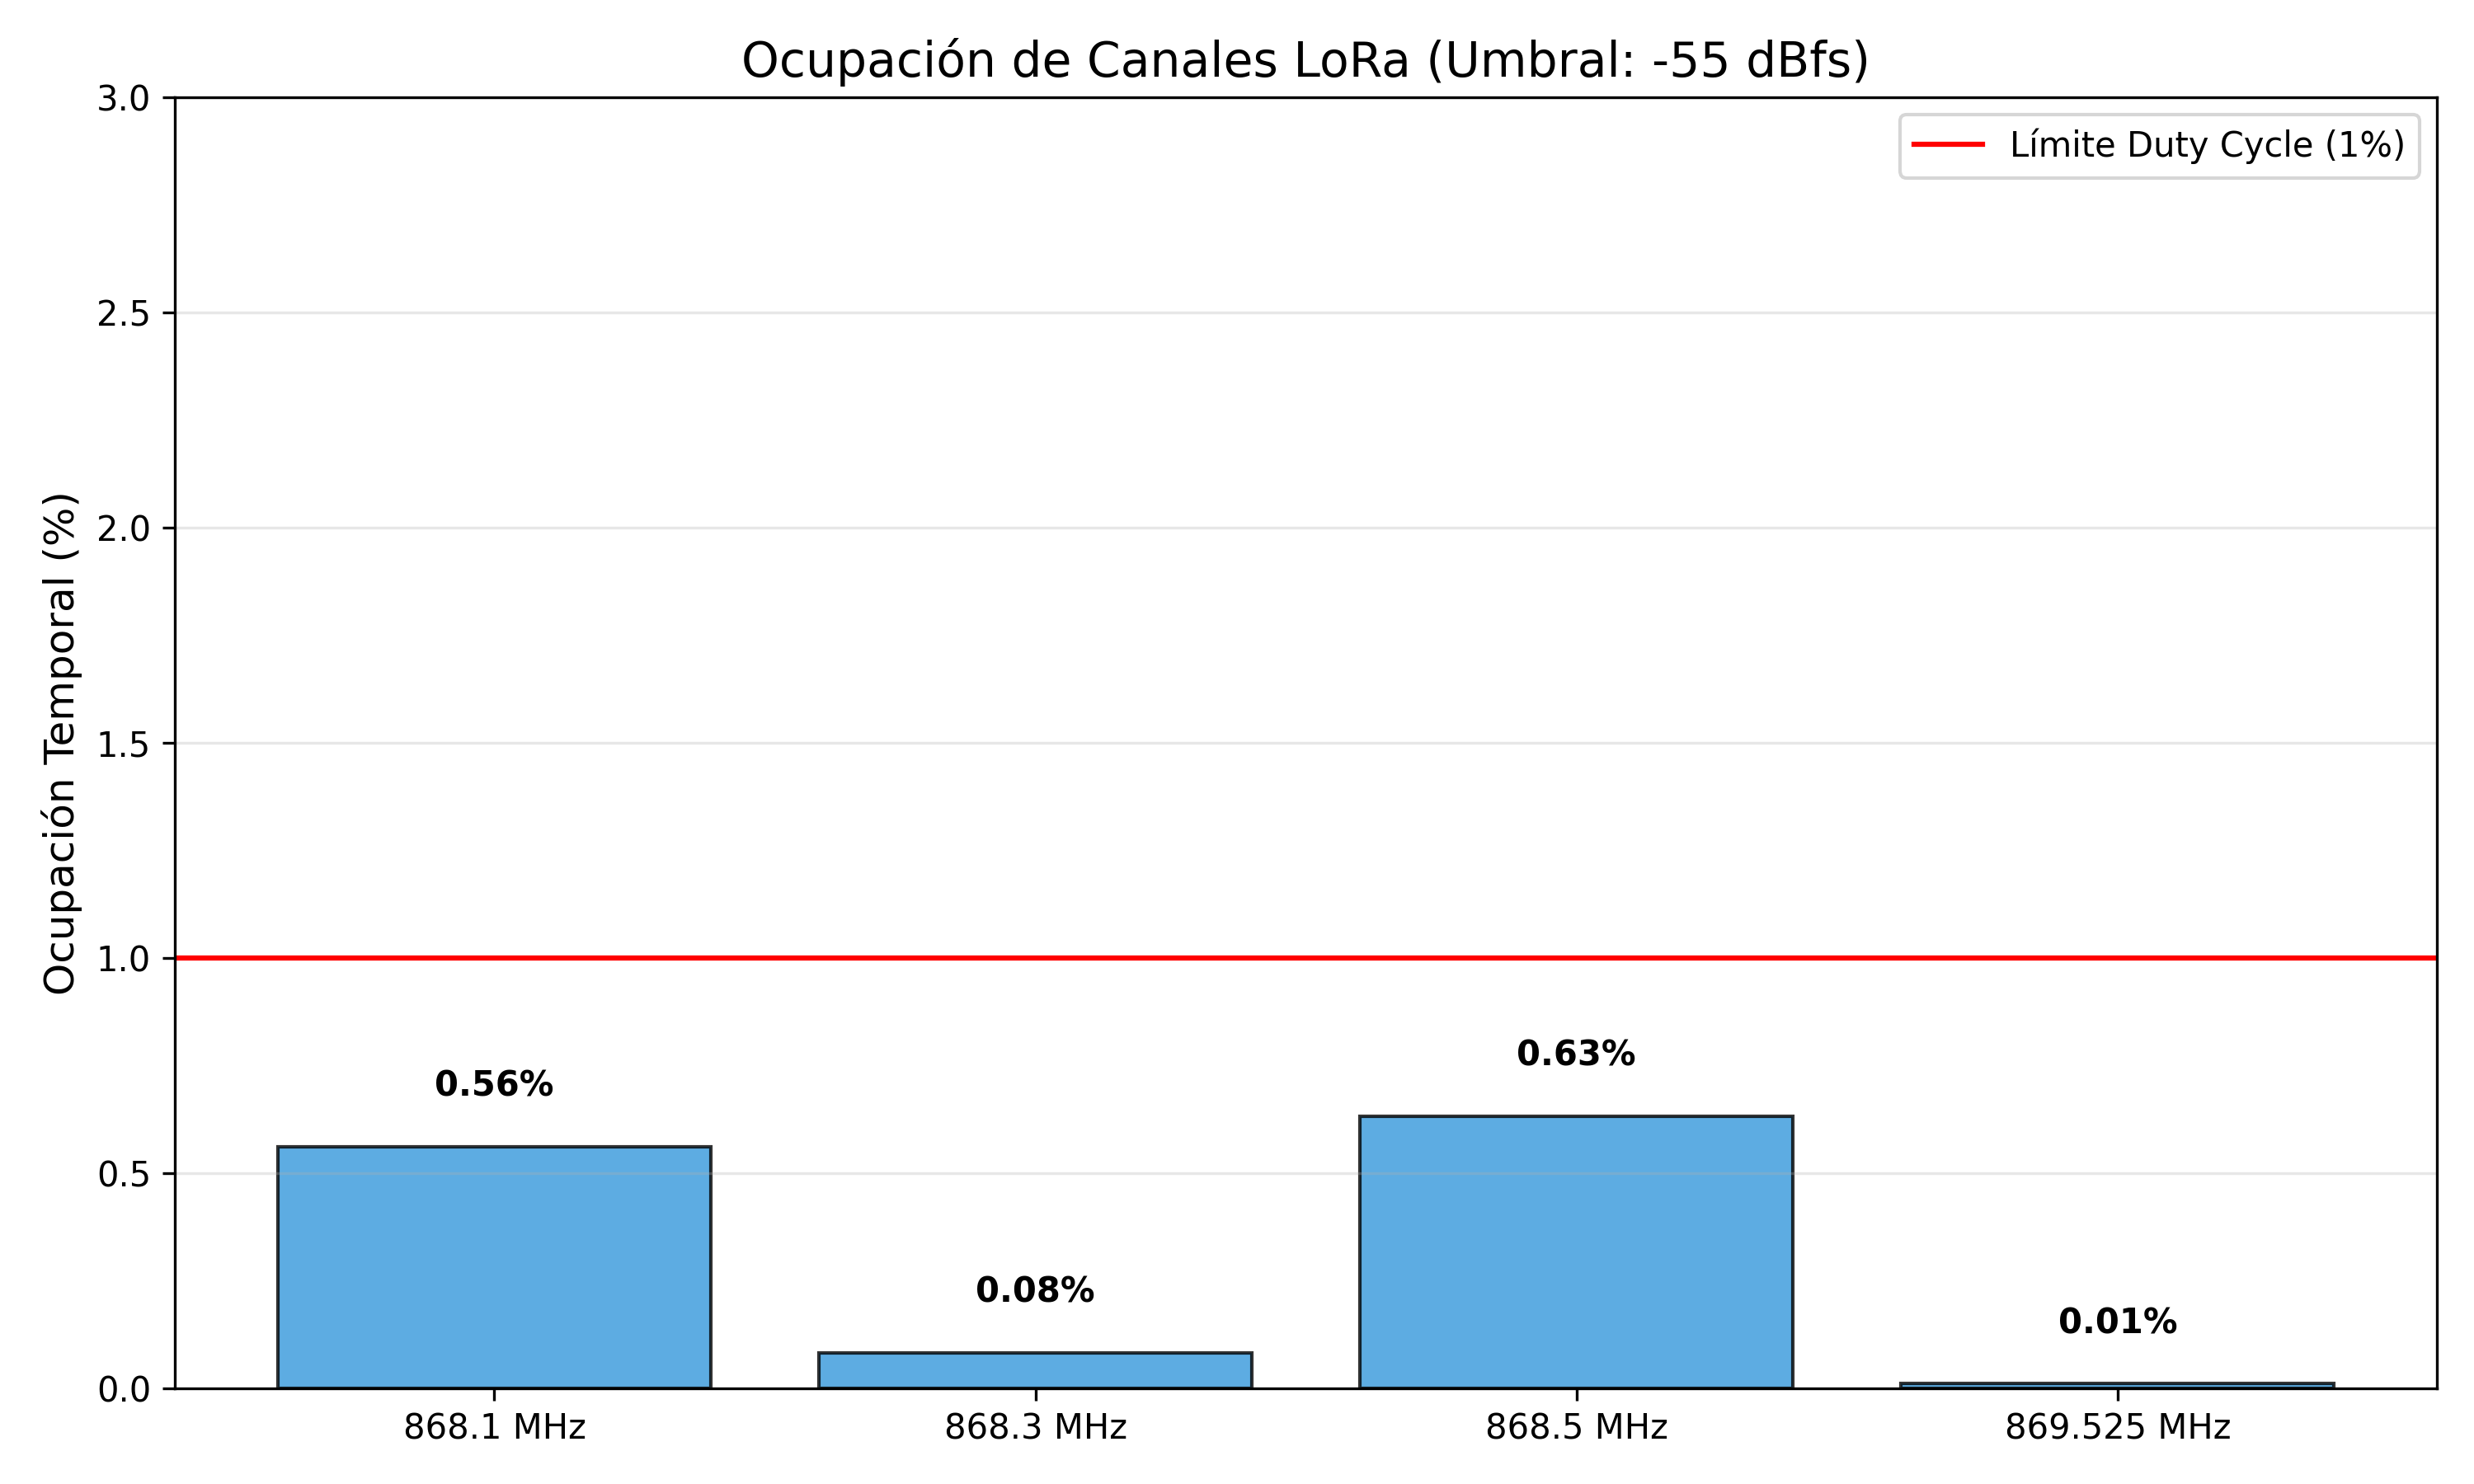
\includegraphics[width=\textwidth]{imagenes/histograma_ocupacion_lora_prueba.png}
\caption{\label{fig:DC} Gráfica de ocupación media de las distintas bandas disponibles.}
\end{figure}

Como se observa en la Figura~\ref{fig:espectro}, el piso de ruido es uniforme en toda la banda, en torno a $-67$~dBFS. La única actividad claramente distinguible del ruido se concentra entre 868,0 y 868,6~MHz, zona en la que se sitúan los canales ascendentes obligatorios de LoRaWAN. Sus picos superan el piso de ruido en más de 40~dB, lo que indica la presencia de transmisores cercanos, y la ocupación medida es de alrededor del 0,5\,\% por canal, como se puede observar en la Figura~\ref{fig:DC}.

En el resto de la banda el valor máximo no se separa del ruido: no se registró ninguna emisión apreciable durante la hora de captura. En particular, en la sub-banda de 869,4--869,65~MHz la ocupación es dos órdenes de magnitud inferior a la de los canales LoRaWAN y corresponde a picos de ruido.

Ante estos resultados, se selecciona como canal de operación la frecuencia de \textbf{869,525~MHz}, situada en la sub-banda de 869,4--869,65~MHz. Esta elección se debe a que ofrece un ciclo de trabajo mayor (máx. 10\,\%, frente al 1\,\% de la sub-banda de 868,0--868,6~MHz) y a que evita los canales que utiliza el tráfico LoRaWAN.

No obstante, esta elección conlleva un riesgo. La frecuencia seleccionada es también la que LoRaWAN emplea por defecto en su segunda ventana de recepción descendente, con SF12, por lo que, si el gateway LoRaWAN cercano la utilizase, interferiría con la red, aunque la captura no registró emisiones en ella.

\section{Viabilidad del proyecto}\label{sec:viabilidad}

Desde el punto de vista técnico, el proyecto es viable gracias a la disponibilidad de transceptores LoRa, hardware de bajo coste (microcontroladores y sensores) y herramientas de desarrollo software. El escenario de implementación, con unas veinte aulas y distancias reducidas, permite abordar el desarrollo sin requisitos exigentes de cobertura o consumo energético. Aun así, el funcionamiento deberá validarse mediante las pruebas previstas durante la implementación.

En cuanto a la viabilidad legal, la frecuencia seleccionada, 869,525~MHz, pertenece a una sub-banda que permite un ciclo de trabajo de hasta el 10\,\%. Su utilización queda condicionada al cumplimiento de los límites de potencia y del resto de requisitos radioeléctricos aplicables.

Por último, la viabilidad económica se apoya en el uso de componentes de bajo coste y herramientas de software libre, así como en la posibilidad de alojar el servidor y la base de datos en el gateway que se ejecutará sobre una Raspberry Pi. El coste definitivo del despliegue dependerá de los componentes seleccionados y de las necesidades de instalación del conjunto de nodos. En el Anexo~\ref{anexo_B} se recoge el presupuesto estimado para implementar un nodo y el gateway.